\section{Overview}
\label{sec: overview}%
In this section, a general description of the architecture of the \verb|CKB| system is provided.
The main aspects of the design are:
\begin{itemize}
    \item \textbf{Client-Server architecture. } It consists of a presentation tier, an application and a data tier.
    The firsts one allow the user to communicate with the server and shows him through the UI the answers it receives back from the application tier.
    The second one receives requests from users, elaborates answers, changes the status communicating with the data tier and sends back the needed information to users.
    Finally, the data tier stores, updates, and handles the information.
    \item \textbf{Microservices. } Functionalities of the system are divided into several services in order to reduce dependencies between
    modules and to increase scalability, availability and maintainability of the system.
\end{itemize}

\section{Component View}
\label{sec: component_view}%
The component diagram shows all the identified components.
It also describes the relations between the modules, representing the verse of the communication flow and the actors participating.

Bla bla bla

\subsection{Component diagram}
\label{subsec:component_diagram}%
\begin{figure} [H]
    \begin{center}
        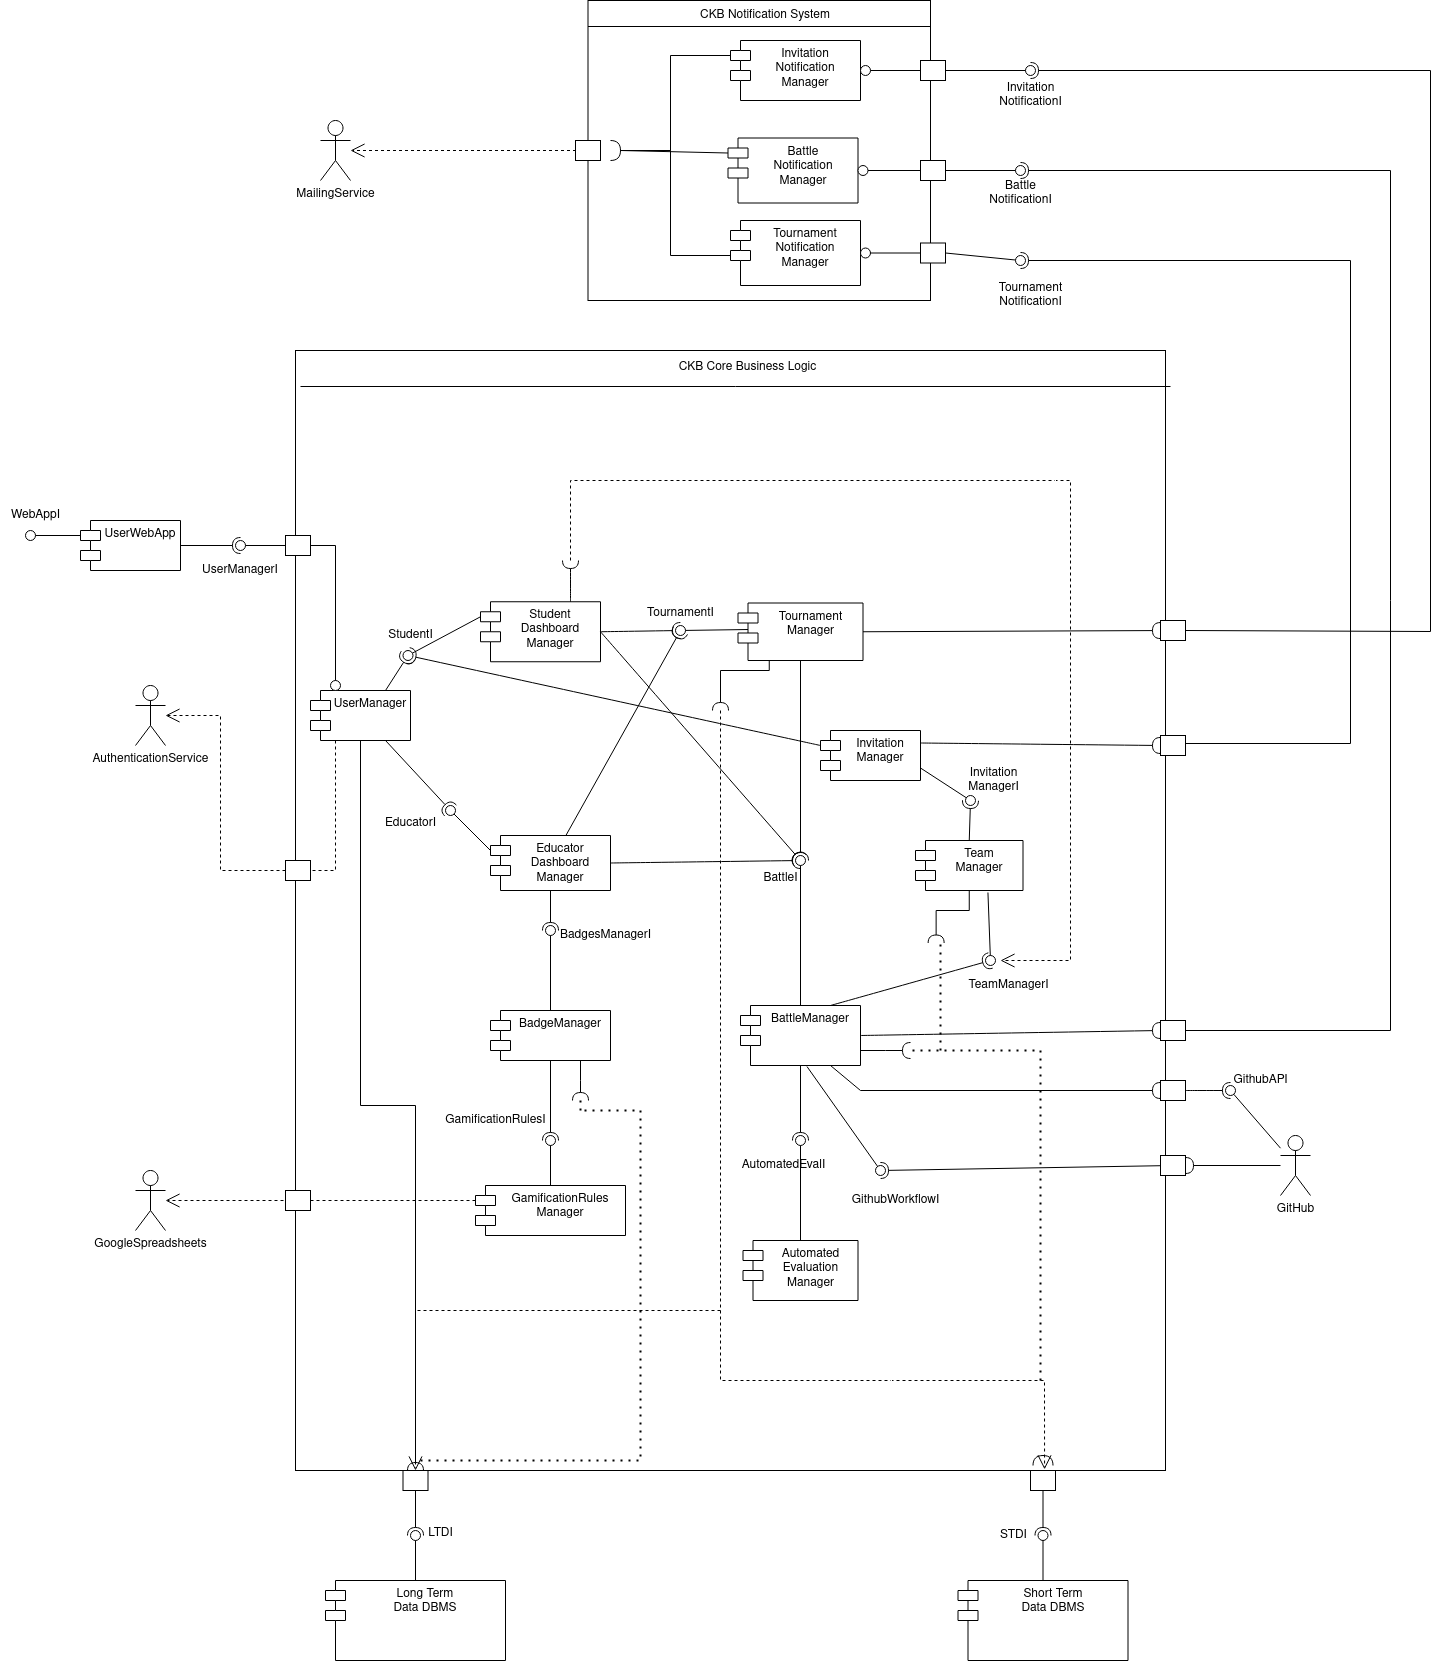
\includegraphics[width=1\linewidth]{Images/compdiag.png}
        \caption{Component diagram of the CKB platform.}
        \label{fig: cd}
    \end{center}
\end{figure}

\subsection{Components description}
\label{subsec:components_description}%
The components are:
\begin{itemize}
    \item \textbf{User WebApp.} \verb|User| \verb|WebApp| is the front-end for users. 
    %It allows them to interact with the system by offering the following functions through the interface UserAppI:
    %    \begin{itemize}
    %        \item \textbf{Register} 
    %        \item \textbf{Login} 
    %        \item \textbf{A} 
    %        \item \textbf{Z} 
    %        \item \textbf{Z} 
    %        \item \textbf{Z} 
    %        \item \textbf{Z} 
    %        \item \textbf{Z} 
    %    \end{itemize}
    \item \textbf{UserManager} \verb|UserManager| component offers, through the interface \verb|UserManagerI|, the basic function for handling users:
        \begin{itemize}
            \item \textbf{Register}
            \item \textbf{Login}
            %tanta altra roba di sicuro
        \end{itemize}
        It also provides user information to the \verb|EducatorDashboardManager| component and the \verb|StudentDashboardManager| component depending on the role of the logged user.
    %EducatorDashboardManager
    \item \textbf{Educator Dashboard Manager.} \verb|Educator| \verb|Dashboard| \verb|Manager| handles the main functionalities accessible by an Educator. 
    It allows creating and managing both CodeKataBattles and Tournaments, defining new badges and rules and performing all the operations that an Educator should be able to perform according to the RASD.
    \item \textbf{Badge Manager.} \verb|Badge| \verb|Manager| is used to manage badges, allowing to perform operations such as assigning a badge to a Student, creating new badges and defining new rules and variables to obtain them.
    \item \textbf{Gamification Rules Manager.} \verb|Gamification| \verb|Rules| \verb|Manager| is used to manage rules and variables used to determine winners of badges. 
    This component relies on an external actor, Google Spreadsheet, to allow defining new rules in a simple but effective way (Spreadsheet formulas).
    \item \textbf{Student Dashboard Manager.} \verb|Student| \verb|Dashboard| \verb|Manager| handles the main functionalities accessible by a Student.
    It allows joining and participating in CodeKataBattles and Tournaments, checking the status of the ongoing ones and the results of the past ones.
    \item \textbf{Battle Manager.} \verb|Battle| \verb|Manager| is used to manage CodeKataBattles, allowing to perform operations such as creating a new CodeKataBattle, 
    joining an existing one and checking the status of the ongoing ones through its interface \verb|BattleI|.
    \item \textbf{Tournament Manager.} \verb|Tournament| \verb|Manager| is used to manage Tournaments, allowing to perform operations such as creating a new Tournament,
    joining an existing one and checking the status of the ongoing ones through its interface \verb|TournamentI|. Educators can also add other Educators as admin to a tournament they created.
    \item \textbf{Automated Evaluation Manager.} \verb|Automated| \verb|Evaluation| \verb|Manager| is used to manage the automated evaluation of CodeKataBattles assigning scores to teams.
    \item \textbf{Team Manager.} \verb|Team| \verb|Manager| is used to manage teams, allowing to perform operations such as creating a new team, joining an existing one and inviting a student to join a team.
    %invitations manager
    \item \textbf{Notification Manager.} \verb|Notification| \verb|Manager| allows Students to be notified via email when a new CodeKataBattle or Tournament is created or ends. It relies on an external Mailing Service.
\end{itemize}
External entities are:
\begin{itemize}
    \item \textbf{Google Spreadsheet.} \verb|Google| \verb|Spreadsheets| is the engine used by Educators when creating new rules for badges. 
    \item \textbf{Mailing Service.} \verb|Mailing| \verb|Service| is used to send emails to Students when a new CodeKataBattle or Tournament is created or ends.
    \item \textbf{Github.} \verb|Github| interacts with the \verb|Battle| \verb|Manager| component to handle the code that represents the solution of a CodeKataBattle. 
    CKB platform offers APIs to allow Github Actions Workflow to trigger a pull request to the repository of the solution.
\end{itemize}

\section{Deployment View}
\label{sec: deployment_view}%
The distribution of components capturing the topology of the system is illustrated below by using a deployment diagram.
The system is structured in a multitier architecture.
\newline
\begin{figure} [H]
    \begin{center}
        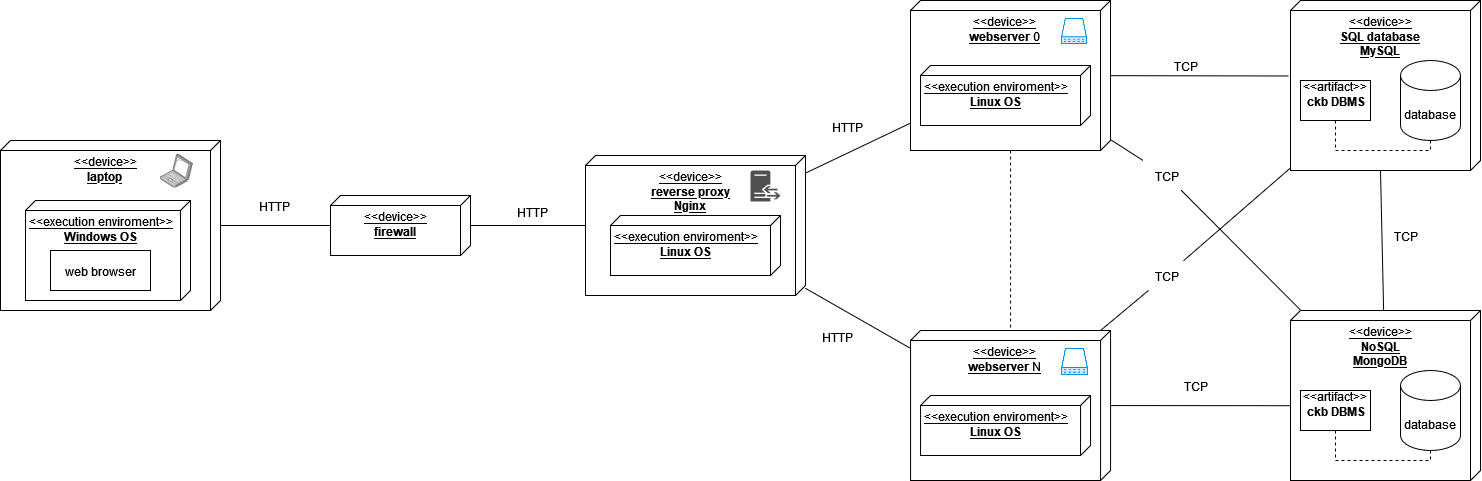
\includegraphics[width=1\linewidth]{Images/deployment_diag.png}
        \caption{Deployment diagram of the CKB platform.}
        \label{fig: depl_diagram}
    \end{center}
\end{figure}


\noindent\textbf{Laptop devices}\newline
This node represents a user's laptop, which is the client-side hardware. The "Windows OS" indicates that the laptop is running on the Windows operating system. 
The "web browser" is the software application used to access the web interface of the platform.

\noindent\textbf{Firewall}\newline
This is a security device that monitors and filters incoming and outgoing network traffic based on an organization's previously established security policies. 
Here, it acts as a barrier between secure internal networks and untrusted external networks, such as the internet.

\noindent\textbf{Reverse Proxy}\newline
This server is running Nginx, which is a web server that can also be used as a reverse proxy. This means it can distribute traffic to various servers, 
thereby acting as an additional layer of abstraction and control to smooth the flow of network traffic between clients and services.

\noindent\textbf{Webserver 0}\newline
This is one of potentially multiple web servers that handle the incoming HTTP requests from the client's web browser, process those requests, 
and serve the appropriate web pages. It runs on a Linux operating system, which suggests a preference for open-source solutions.

\noindent\textbf{Webserver N}\newline
This indicates there are multiple webservers in this deployment, following a similar configuration to "Webserver 0." 
The "N" represents an indefinite number, showing that the architecture is scalable and can include as many webservers as needed.

\noindent\textbf{SQL database (MySQL)}\newline
This database node uses MySQL, which is a relational database management system (RDBMS) based on SQL (Structured Query Language). 
It's used to store and manage the platform's structured data efficiently.

\noindent\textbf{NoSQL database (MongoDB)}\newline
This is a NoSQL database, specifically MongoDB, which is designed for storing unstructured data. It offers high performance, high availability, and easy scalability.

\noindent\textbf{ckb DBMS}\newline
This artifact within both database nodes represents the database management software that's part of the CodeKataBattle platform. It is likely the collection of schemas, 
tables, queries, reports, views, and other objects associated with the platform's database management.